\documentclass{article}
% main document, called main.tex
\usepackage{tikz}
\usetikzlibrary{external}

\usetikzlibrary{positioning}
\usetikzlibrary{calc}
\usetikzlibrary{shapes.geometric, arrows, arrows.meta}
\usepackage{varwidth}% http://ctan.org/pkg/varwidth
\usetikzlibrary{shadows,trees, mindmap}
\usetikzlibrary{matrix}
\usetikzlibrary{fit}

\tikzexternalize % activate!
\begin{document}
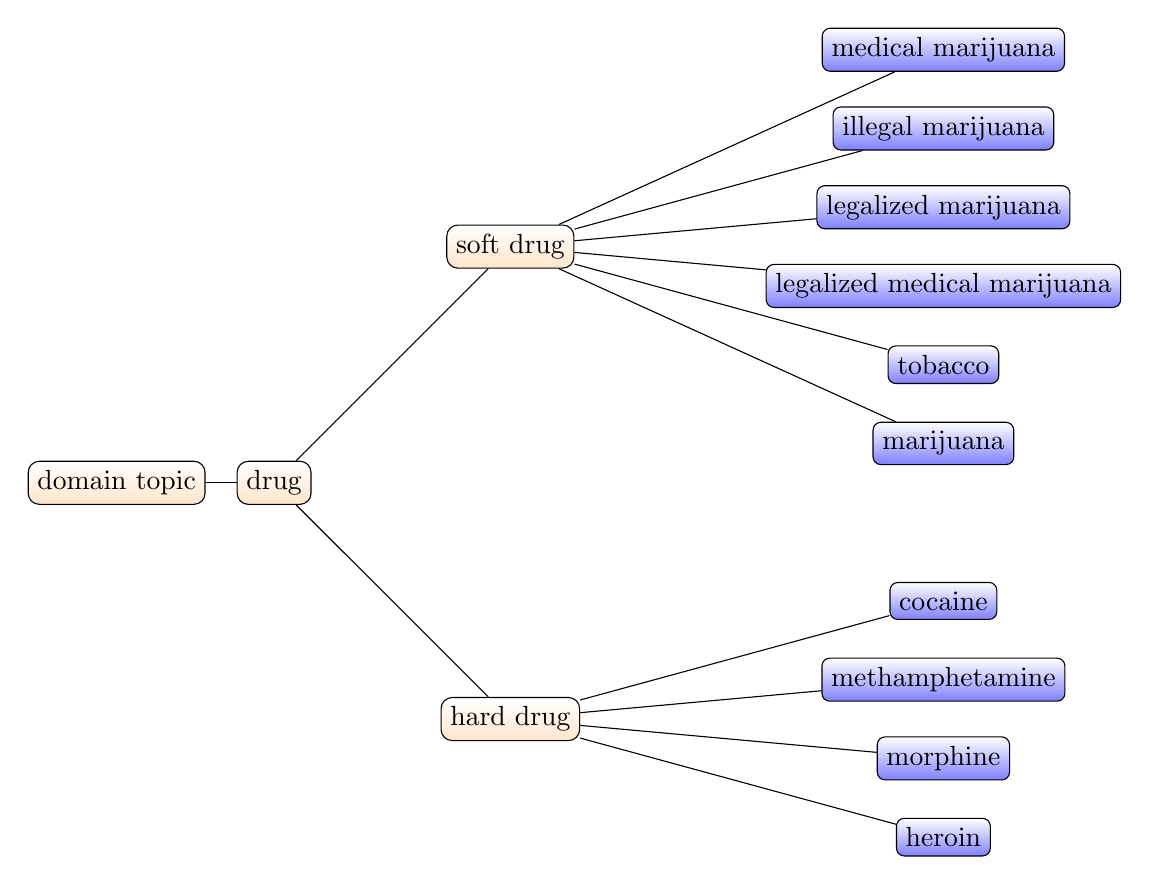
\begin{tikzpicture}
[grow'=right,
level 1/.style={sibling distance=1.5cm, level distance=2cm},
level 2/.style={sibling distance=1.5cm, level distance=3cm, },
level 3/.style={
sibling distance=1cm, level distance=5.5cm},
concept/.style=
{shape=rectangle, rounded corners,
draw, align=center,
top color=white, bottom color=orange!20},
individual/.style={rectangle, rounded corners=1mm, draw, top color=white, bottom color=blue!50,
text centered}
	]
	\node (root) [concept] {domain topic}
	child  { node [concept] {drug}
	child  { node [concept] {soft drug} 
	child { node [individual] {medical marijuana}}
	child { node [individual] {illegal marijuana}}
	child { node [individual] {legalized marijuana}}
	child { node [individual] {legalized  medical marijuana}}
	child { node [individual] {tobacco}}
	child { node [individual] {marijuana}}
    }
    child [missing]
    child [missing]
    child [missing]
    child {node  [concept]{hard drug}
	child {node [individual] {cocaine}}
	child {node [individual] {methamphetamine}}
	child {node [individual] {morphine}}
	child {node [individual] {heroin}}
    }
};
	
\end{tikzpicture}

\end{document}

